\documentclass[12pt]{article}

% Any percent sign marks a comment to the end of the line

% Every latex document starts with a documentclass declaration like this
% The option dvips allows for graphics, 12pt is the font size, and article
%   is the style

\usepackage[pdftex]{graphicx}
\usepackage{amsfonts}
\usepackage{amsmath}
\DeclareMathOperator*{\max_bottom}{max}
\usepackage{url}
\usepackage{hyperref}

\usepackage{caption}
\usepackage{subcaption}

\usepackage{graphicx}
\usepackage{amsmath}
\usepackage{adjustbox}
\usepackage{listings}

\lstset{language=python}

\hypersetup{
    colorlinks=true,
    linkcolor=blue,
    filecolor=magenta,      
    urlcolor=cyan,
    pdftitle={Sharelatex Example},
    bookmarks=true,
    pdfpagemode=FullScreen,
}


\usepackage{graphicx}
\graphicspath{ {./images/} }

% These are additional packages for "pdflatex", graphics, and to include
% hyperlinks inside a document.

\setlength{\oddsidemargin}{0.5cm}
\setlength{\evensidemargin}{0.5cm}
\setlength{\topmargin}{-1.6cm}
\setlength{\leftmargin}{0.5cm}
\setlength{\rightmargin}{0.5cm}
\setlength{\textheight}{24.00cm} 
\setlength{\textwidth}{15.00cm}
\parindent 0pt
\parskip 5pt
\pagestyle{plain}

% These force using more of the margins that is the default style
\newcommand{\namelistlabel}[1]{\mbox{#1}\hfil}
\newenvironment{namelist}[1]{%1
\begin{list}{}
    {
        \let\makelabel\namelistlabel
        \settowidth{\labelwidth}{#1}
        \setlength{\leftmargin}{1.1\labelwidth}
    }
  }{%1
\end{list}}


\begin{document}
\title{\Huge Introduction to machine learning - Homework 3}

\author{
  \textbf{Uri Kirstein}\\
  311137095 \\ sukirstn@campus.technion.ac.il
  \\ \\
  \textbf{Pavel Rastopchin}\\
  321082026 \\ pavelr@campus.technion.ac.il
  \\ \\ 
}

\maketitle


\newpage
\section{Process and significant decisions}
\subsection{Dividing the data to Train set and Test set}
We decided to divide the data to two sets with ratio 0.85:0.15. The train set of 8500 samples will be used during k-fold cross validation and ensemble generation. Then, the final model will be evaluated on 1500 test samples to get the final accuracy of our model and from this point we will not be able to do any changes on our model, as it will be considered as "information leakage" as we changes something in the model based on the test set results. Also, the model will not be trained then on the whole 10000 samples, as based on the articles we found, this is a bad practise. After those steps we will predict the labels of the unlabelled data. The statistics which where used to transform the data in the test set and the unlabelled set were calculated according to train set (8500 samples) only.  

\subsection{Using one model and ensemble technique}
In Homework 3, during the automatic model selection, we found that the best model for the prediction tasks is a Multi-layer perceptron. In this homework we decided to use MLP model as well, according our findings. The main problem with sklearn MLP model was a high level of abstraction which prevented from us to use more advanced techniques. Thus, in this homework we will use Keras framework to build a deep learning model. To boost our model accuracy we decided to use ensemble technique. We will train multiple MLP models, then use all of them to predict the labels. 

\subsection{Hyper parameters tuning with random search}
Based on Stanford CS231n course, lectures 6,7, we decided to use another technique for tuning the MLP parameters using random search, as this "brute force" technique might achieve better results than tuning parameters one by one. In all our cross-validation experiments we used the $accuracy$ and $f1$ score as model performance measurement. Models which achieve more than 0.945 on average with both metrics will be trained on whole training set and then saved and used as a part of ensemble.

\begin{figure}[h]
\centering
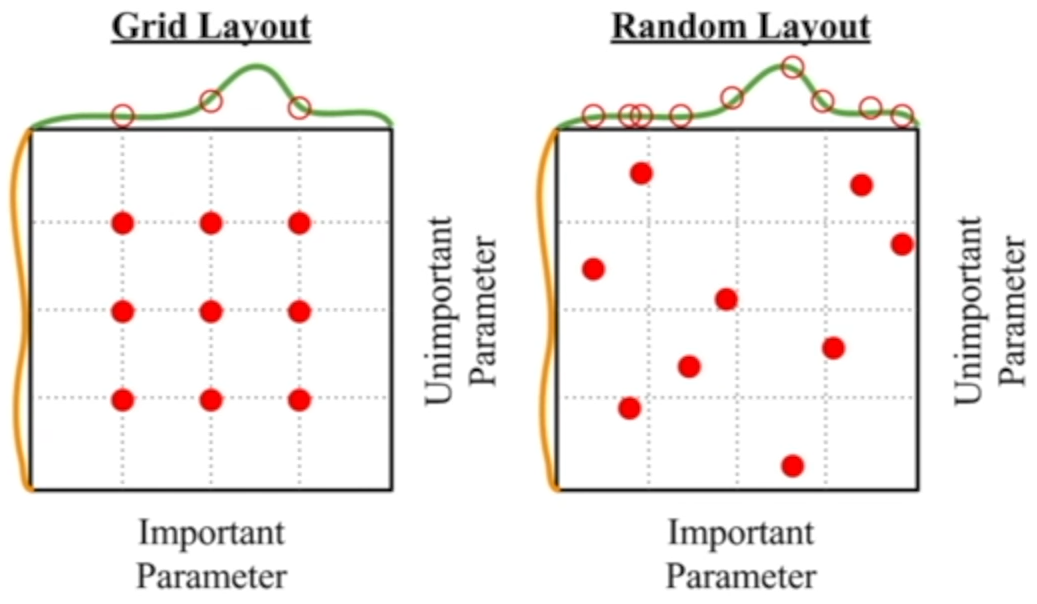
\includegraphics[width=.6\linewidth]{pics/random_search}
\caption{Random search of hyper-parameters}
\end{figure}

\section{MLP hyper-parameters tuning by random search}
\subsection{Dropout probability}
Dropout is a regularization technique for reducing overfitting in neural networks by preventing complex co-adaptations on training data. The term "dropout" refers to dropping out units in a neural network. During the Random search we will draw a random number from 0.01 to 0.6 and this will be the dropout probability in a current model. 
\subsection{Activation functions}
We will draw randomly the activation functions for each model. The options are ReLU, Leaky ReLU and tanh, while for Leaky ReLU we also draw a slope of the negative part of the function from 0.01 to 0.5.
\subsection{Number of hidden layers and their sizes}
For current data-set, deep neural networks tend to over-fit, thus we will draw a random number of hidden layers from 0 to 5, and for each layer a number of neurons from 5 to 200 (based on our finding in HW3).
\subsection{Batch Normalization}
For each model we will decide randomly either to use or not batch normalization between the layers. 

\newpage
\section{Cross validation Results}
During the cross validation we've trained more than 1200 models with different performance and maintained a log which contains the hyper parameters. As we can see in the plot, some models reached higher scores than the target value. Those models were retrained on whole train set and saved as model file. In total producing 11 models with cross validation average accuracy of 0.948 to 0.953.

\begin{figure}[h]
\centering
\includegraphics[width=\linewidth]{pics/randsrc}
\caption{Random search performance}
\end{figure} 

It's worth to mention that we loved a lot this technique as the process fully automated and does not require any manual involvement. We've just prepared the data and gave the code to run over few days. It's a brute-force, lazy-technique which achieved incredibly high final score, much higher than the MLP model with manually tuned hyper-parameters in HW3. 

\newpage
\section{Validation results and Final predictions}
\subsection{Validation set accuracy}
When the ensemble of 11 models was ready, we tested it's performance on 1500 samples set which was never seen by any of the models. The accuracy of the ensemble on the test set is: 0.954.

\subsection{Predicted Winner}
\begin{verbatim}
Winner prediction -  Browns  party will win the elections.
\end{verbatim}

\subsection{Predicted Votes division}
\begin{verbatim}
Prediction - Vote division:
Party  Browns : 20.94 %
Party  Purples : 20.83 %
Party  Blues : 9.97 %
Party  Pinks : 8.66 %
Party  Greens : 8.36 %
Party  Oranges : 7.51 %
Party  Greys : 5.57 %
Party  Yellows : 4.84 %
Party  Whites : 4.51 %
Party  Reds : 4.43 %
Party  Turquoises : 3.38 %
Party  Khakis : 0.78 %
Party  Violets : 0.22 %
\end{verbatim}

\subsection{Conclusion}
As we can see, the Browns party will win the elections with difference of $0.11\%$ which is 11 votes in total. What a close race! 


\end{document}


\begin{figure}[h]
\centering
\begin{subfigure}{.5\textwidth}
  \centering
  \includegraphics[width=.6\linewidth]{Cross_valid_plots/SVM_C_hyper_fig_coarse.png}
  \caption{C coarse tuning}
  \label{fig:sub1}
\end{subfigure}%
\begin{subfigure}{.5\textwidth}
  \centering
  \includegraphics[width=.6\linewidth]{Cross_valid_plots/SVM_C_hyper_fig_fine.png}
  \caption{C fine tuning}
  \label{fig:sub2}
\end{subfigure}
\caption{Random search}
\label{fig:test}
\end{figure}

